\documentclass[a4paper, 12pt]{article}%тип документа

%отступы
\usepackage[left=2cm,right=2cm,top=2cm,bottom=3cm,bindingoffset=0cm]{geometry}

%Русский язык
\usepackage[T2A]{fontenc} %кодировка
\usepackage[utf8]{inputenc} %кодировка исходного кода
\usepackage[english,russian]{babel} %локализация и переносы

%Вставка картинок
\usepackage{wrapfig}
\usepackage{graphicx}
\graphicspath{{pictures/}}
\DeclareGraphicsExtensions{.pdf,.png,.jpg}

%оглавление
\usepackage{titlesec}
\titlespacing{\chapter}{0pt}{-30pt}{12pt}
\titlespacing{\section}{\parindent}{5mm}{5mm}
\titlespacing{\subsection}{\parindent}{5mm}{5mm}
\usepackage{setspace}

%Графики
\usepackage{multirow}
\usepackage{pgfplots}
\pgfplotsset{compat=1.9}

%Математика
\usepackage{amsmath, amsfonts, amssymb, amsthm, mathtools}

\begin{document}

\begin{titlepage}

\begin{center}
%\vspace*{1cm}
\large\textbf{Московский Физико-Технический Институт}\\
\large\textbf{(государственный университет)}
\vfill
\line(1,0){430}\\[1mm]
\huge\textbf{Работа 20}\\
\line(1,0){430}\\[1mm]
\vfill
\large Сибгатуллин Булат, ФРКТ\\
\end{center}

\end{titlepage}

\section{Система с индуктивной связью}

\begin{enumerate}

\item Откроем файл 2LCM.CIR, изучим схему данной системы с индуктивной связью.

\begin{figure}[h!]
\centering
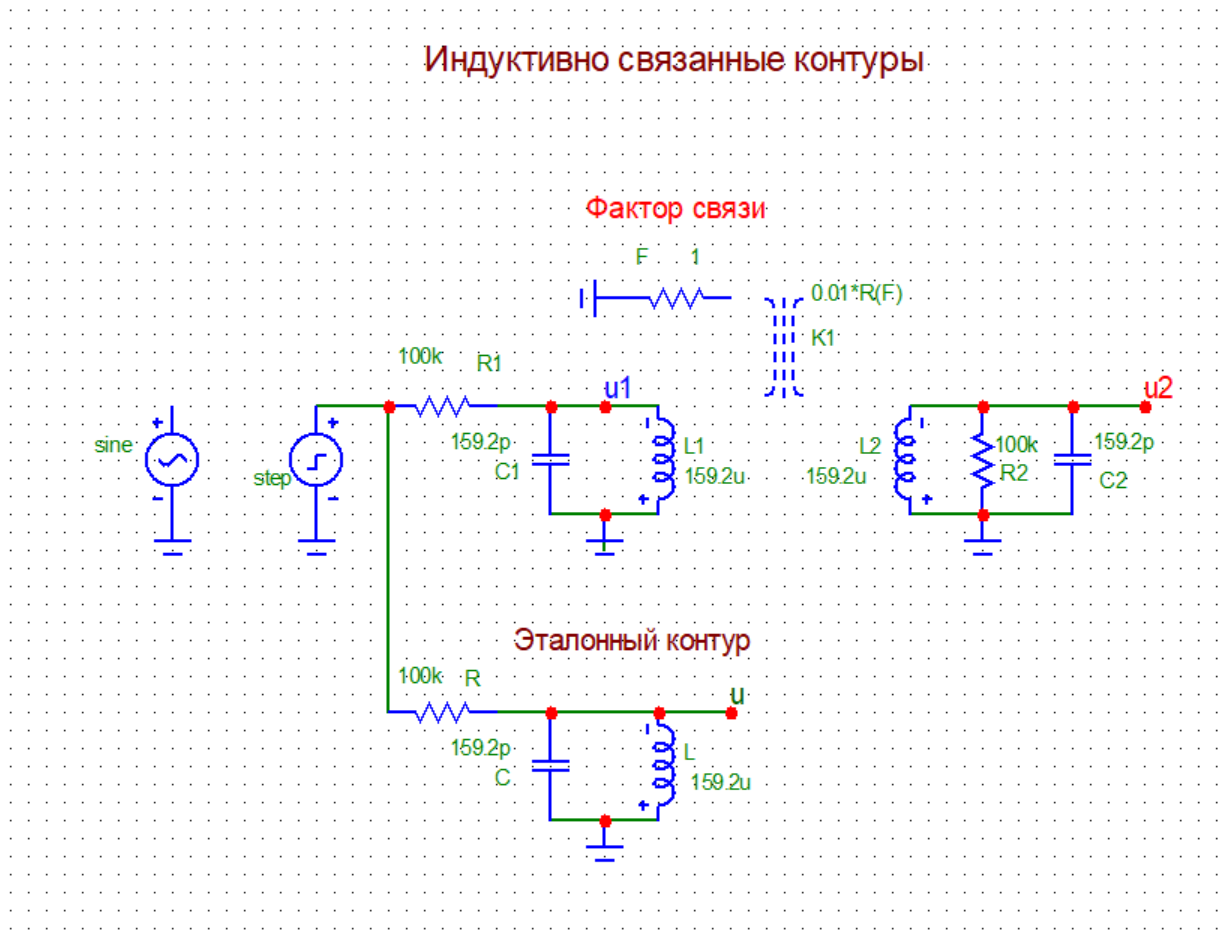
\includegraphics[scale = 0.7]{images/2LCM.png}
\label{fig:Image1}
\end{figure}

\item Оставим только \textbf{плот 2} - просто частотные характеристики схемы. Посмотрим на поведение схемы при варьировании параметров контуров при критической связи.

\begin{figure}[h!]
\centering
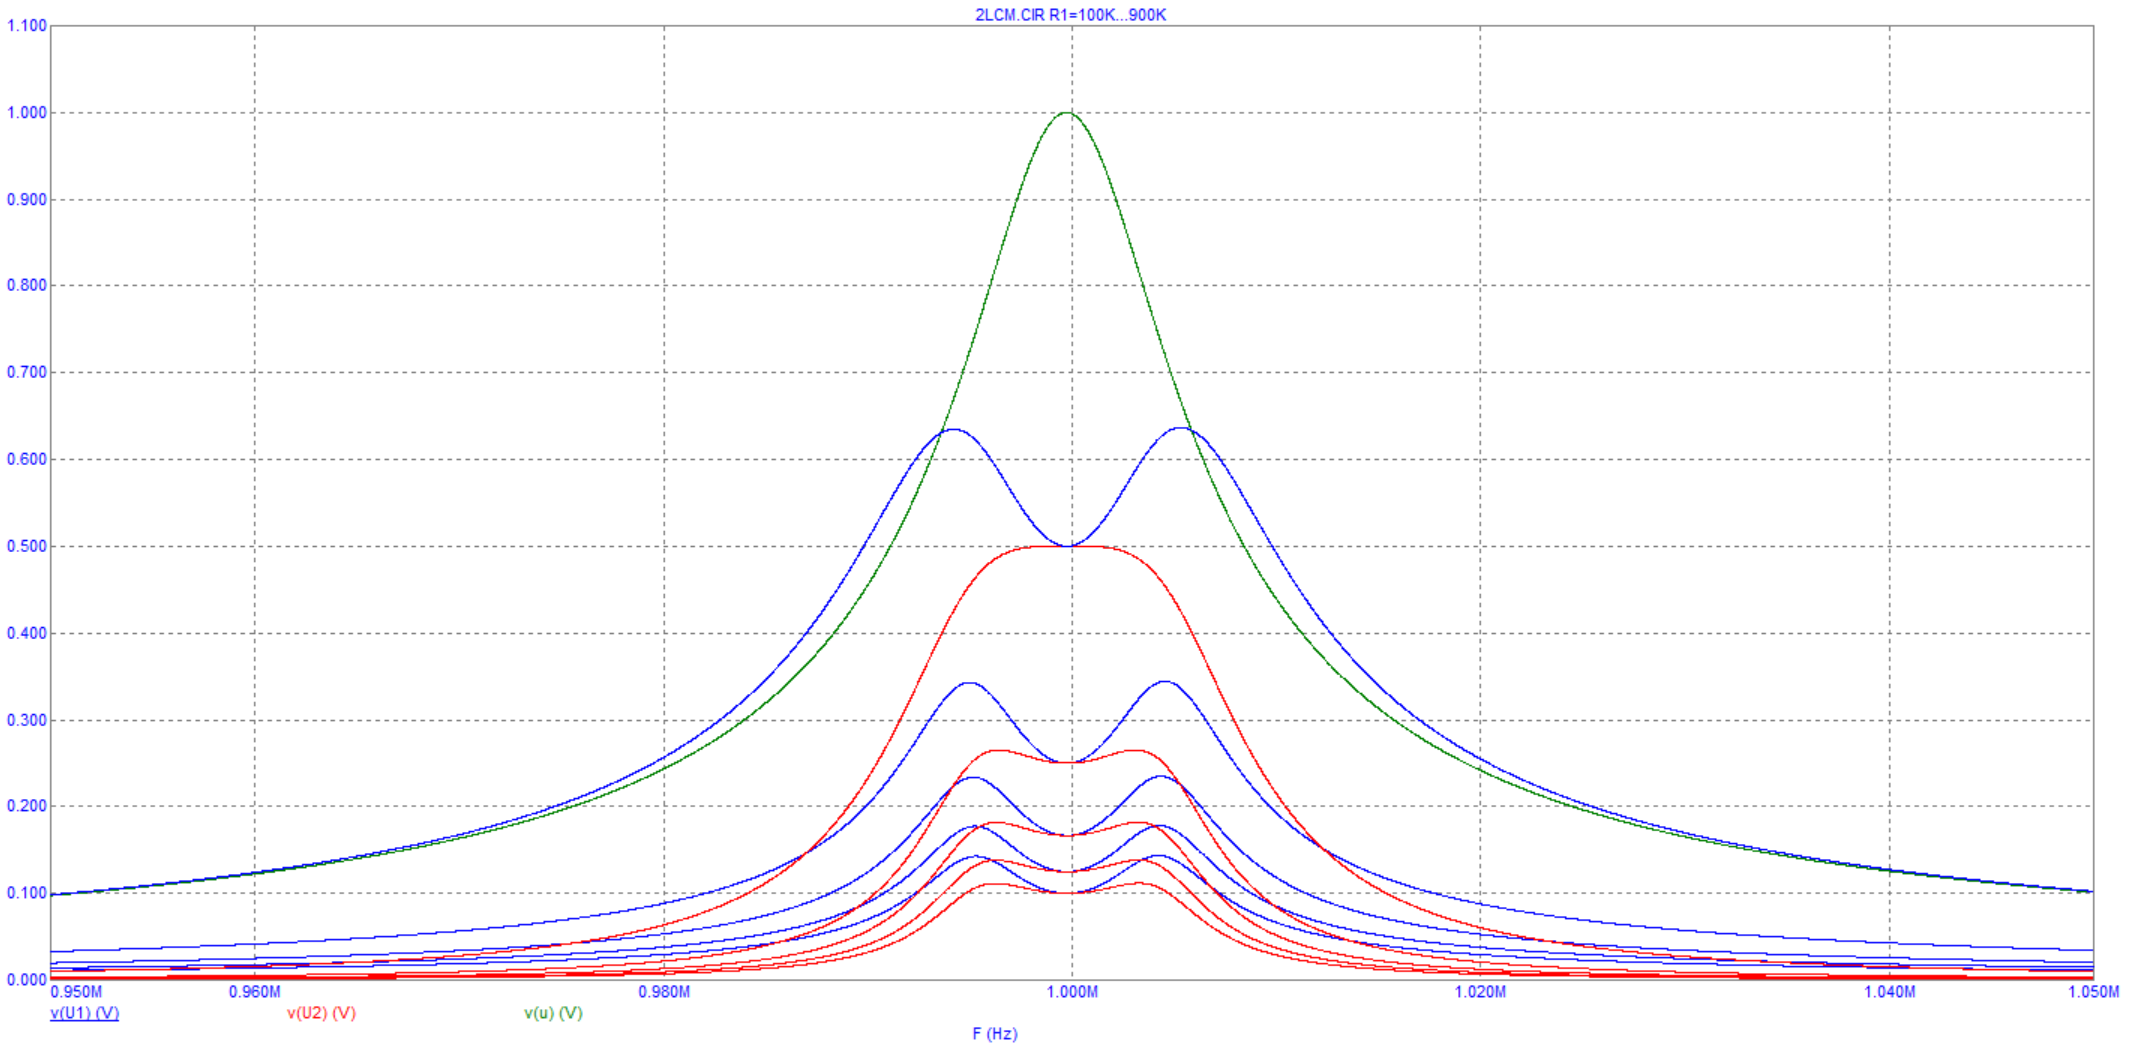
\includegraphics[scale = 0.4]{images/plot2_1.png}
\caption{$R_1 = [100k, 900k|200k], \: R_2 = 100k$}
\label{fig:Image1}
\end{figure}

\begin{figure}[h!]
\centering
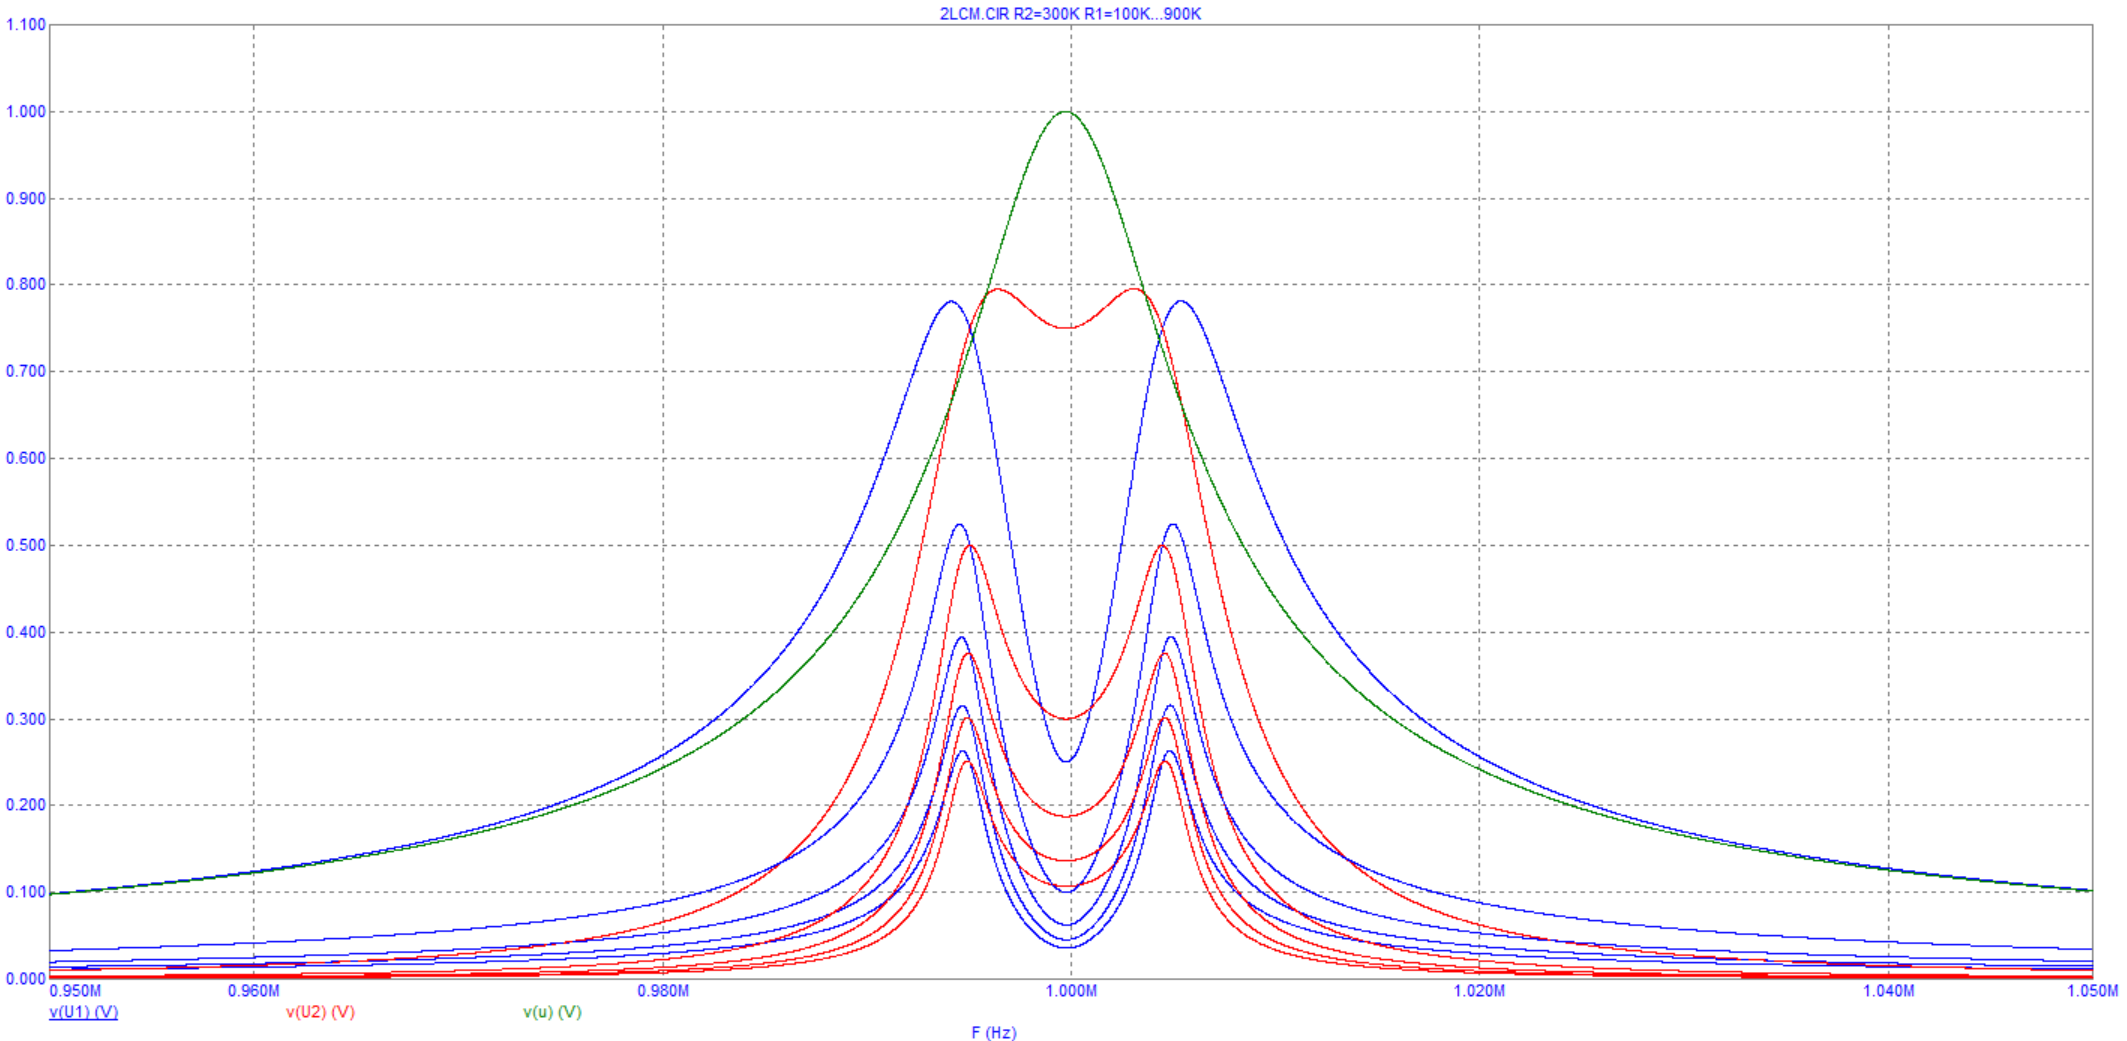
\includegraphics[scale = 0.4]{images/plot2_2.png}
\caption{$R_1 = [100k, 900k|200k], \: R_2 = 300k$}
\label{fig:Image1}
\end{figure}

\begin{figure}[h!]
\centering
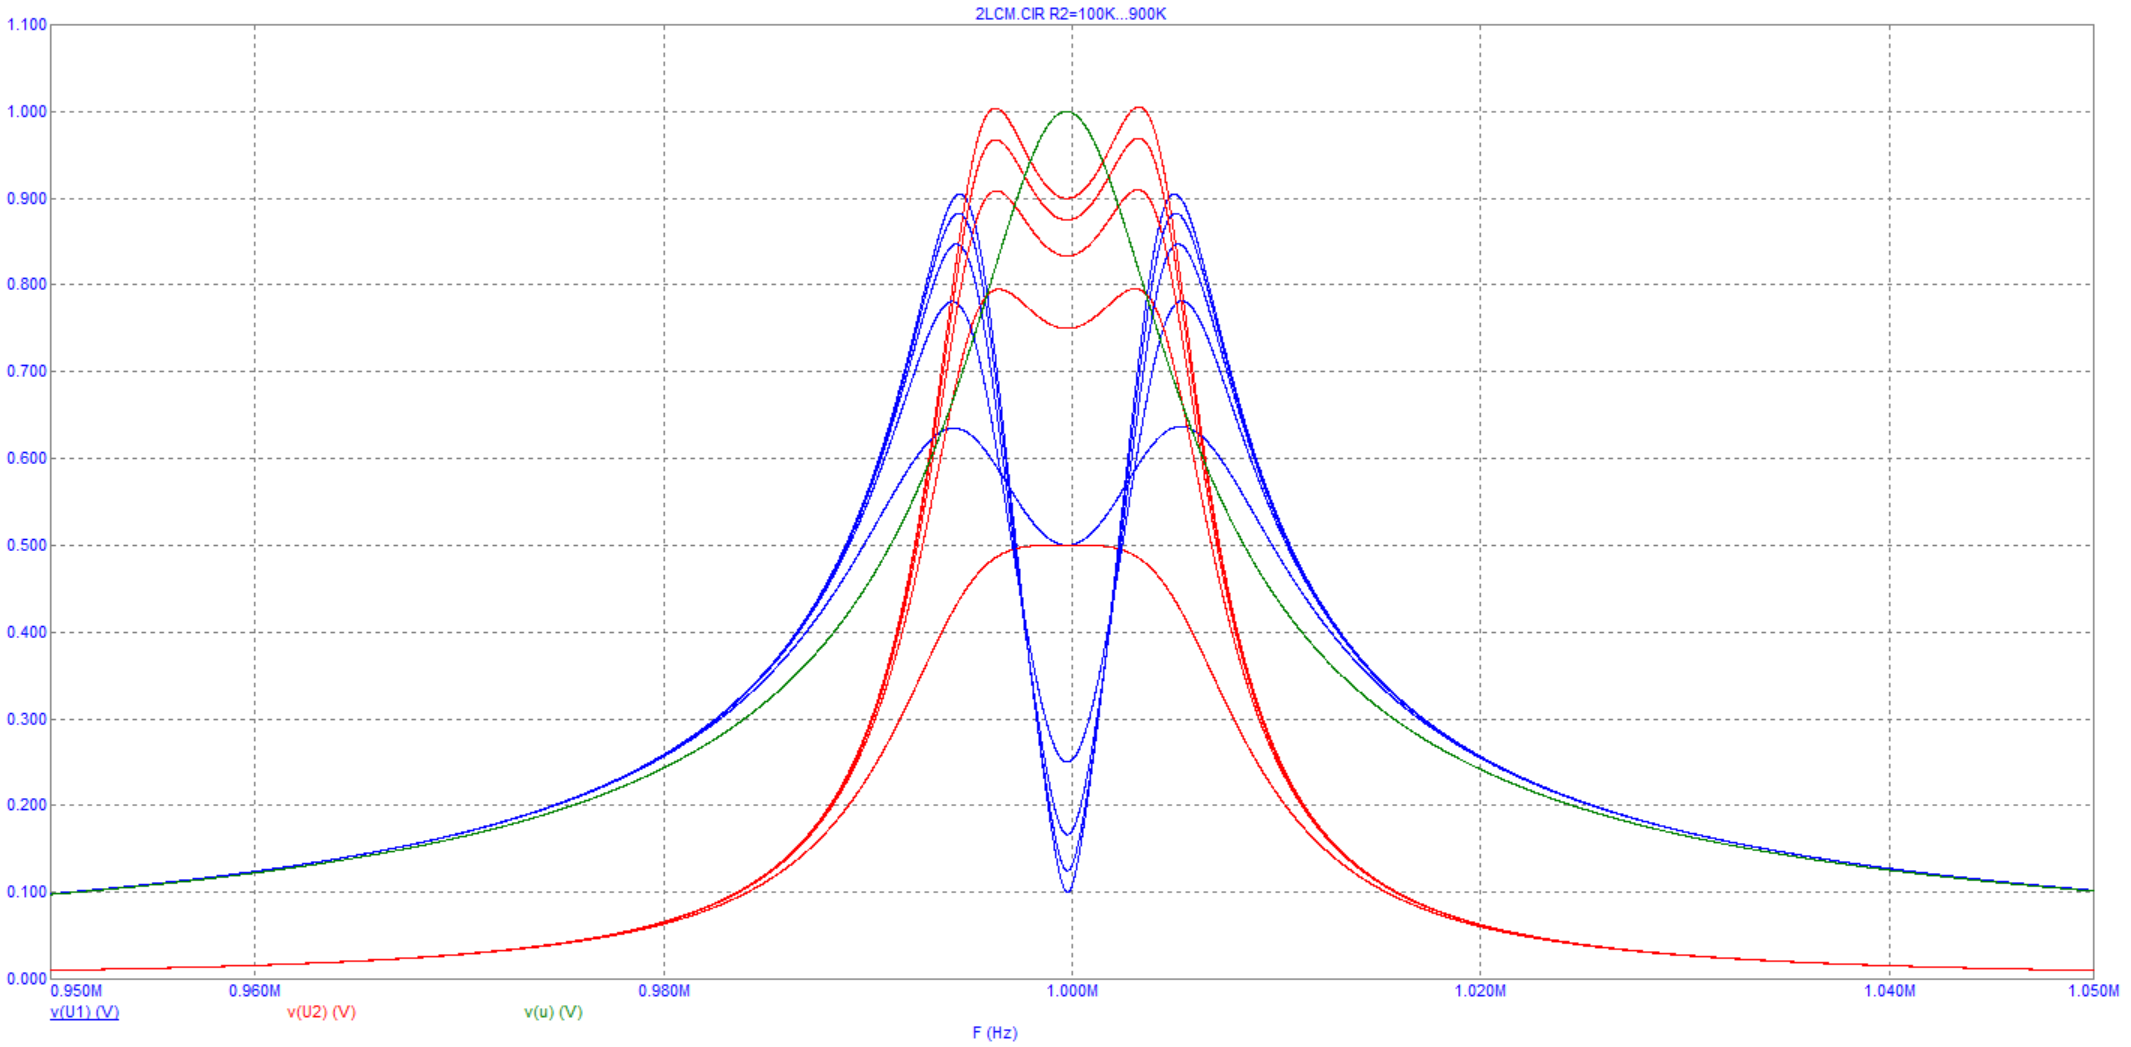
\includegraphics[scale = 0.4]{images/plot2_3.png}
\caption{$R_1 = 100k, \: R_2 = [100k, 900k|200k]$}
\label{fig:Image1}
\end{figure}

\begin{figure}[h!]
\centering
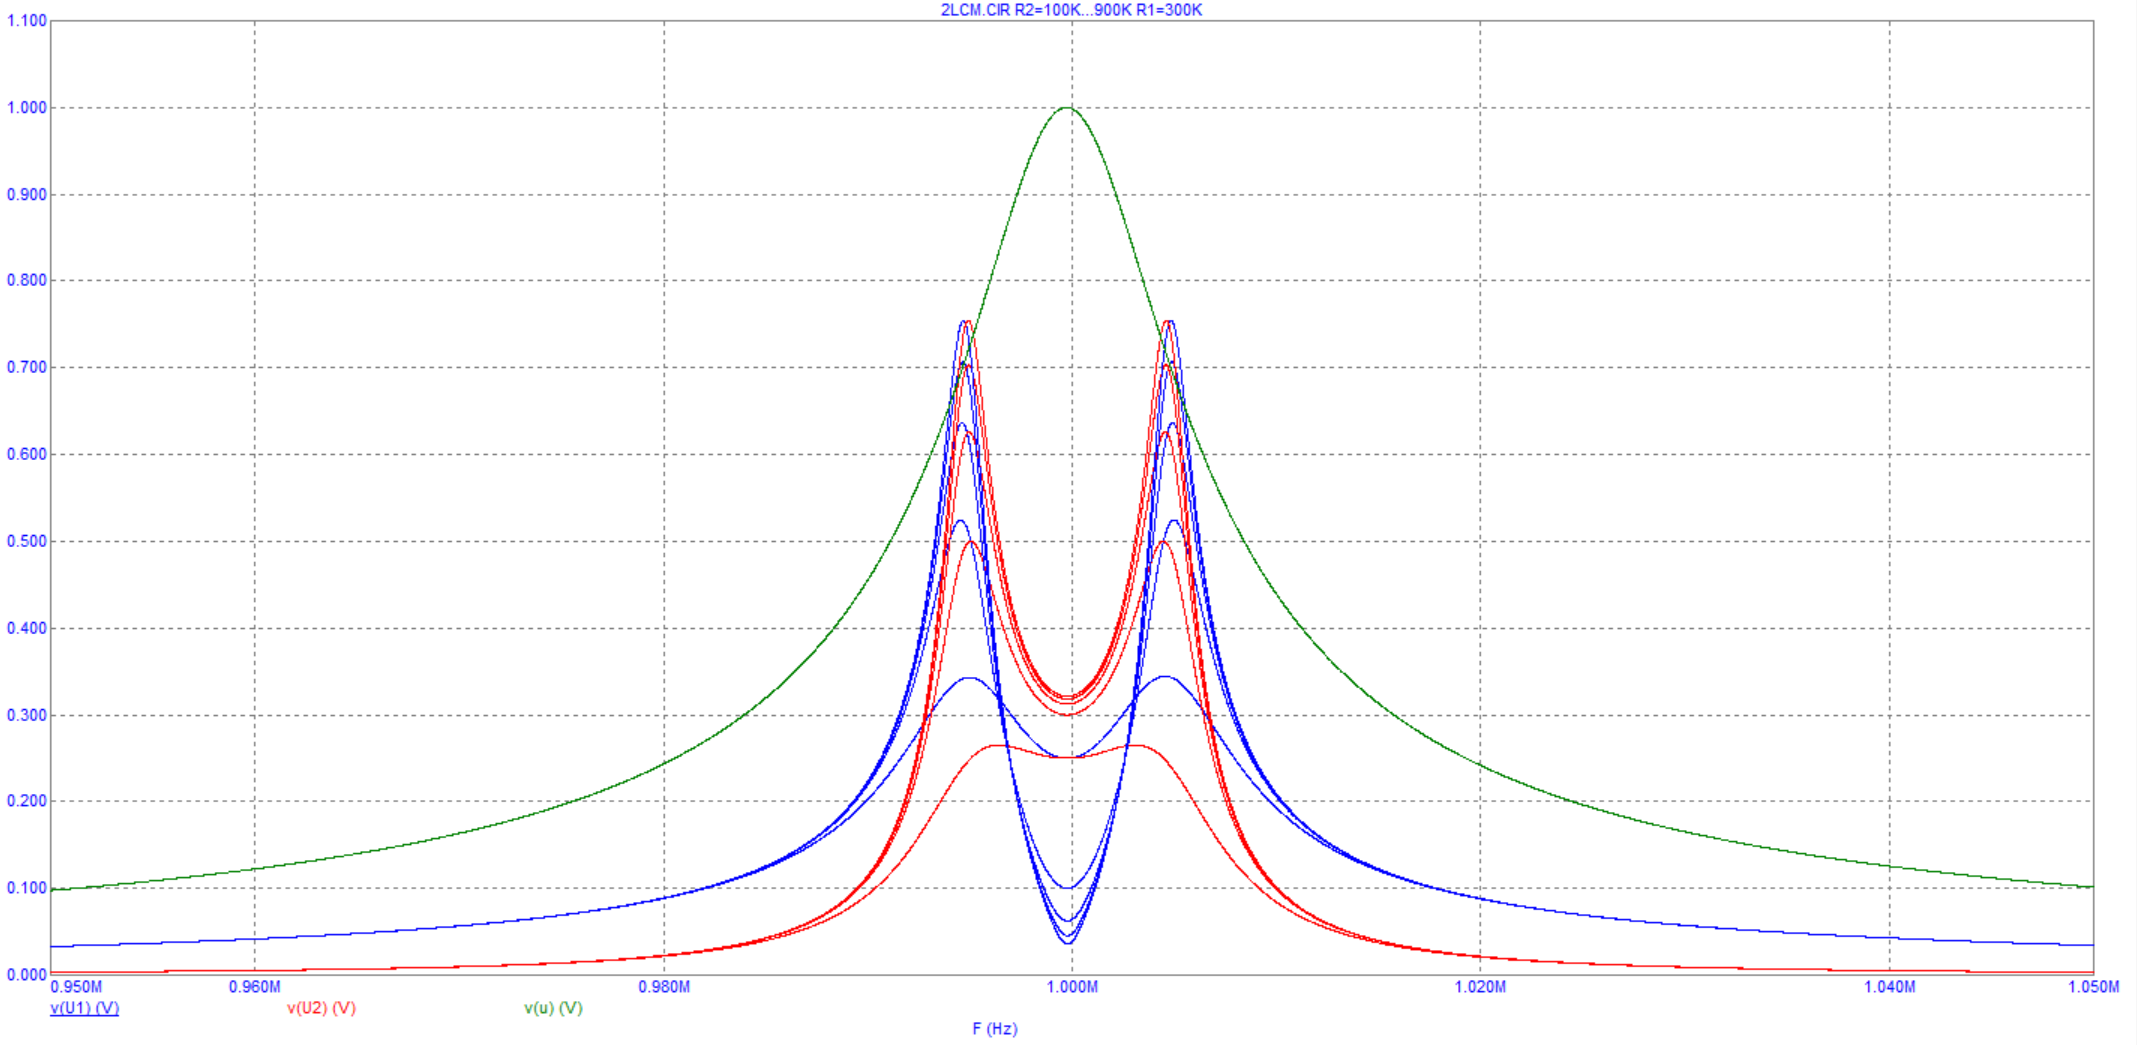
\includegraphics[scale = 0.4]{images/plot2_4.png}
\caption{$R_1 = 300k, \: R_2 = [100k, 900k|200k]$}
\label{fig:Image1}
\end{figure}

\end{enumerate}

\end{document}
